%  Copyright 2020-2022 Robert Bosch GmbH
%
%  Licensed under the Apache License, Version 2.0 (the "License");
%  you may not use this file except in compliance with the License.
%  You may obtain a copy of the License at
%
%      http://www.apache.org/licenses/LICENSE-2.0
%
%  Unless required by applicable law or agreed to in writing, software
%  distributed under the License is distributed on an "AS IS" BASIS,
%  WITHOUT WARRANTIES OR CONDITIONS OF ANY KIND, either express or implied.
%  See the License for the specific language governing permissions and
%  limitations under the License.
%
\documentclass[a4paper,10pt]{report}

% --------------------------------------------------------------------------------------------------------------
% common preamble
% --------------------------------------------------------------------------------------------------------------

% --------------------------------------------------------------------------------------------------------------
%
% Copyright 2020-2022 Robert Bosch GmbH

% Licensed under the Apache License, Version 2.0 (the "License");
% you may not use this file except in compliance with the License.
% You may obtain a copy of the License at

% http://www.apache.org/licenses/LICENSE-2.0

% Unless required by applicable law or agreed to in writing, software
% distributed under the License is distributed on an "AS IS" BASIS,
% WITHOUT WARRANTIES OR CONDITIONS OF ANY KIND, either express or implied.
% See the License for the specific language governing permissions and
% limitations under the License.
%
% --------------------------------------------------------------------------------------------------------------
%
% preamble.tex
%
% Common preamble for tex files (used for both: GenPackageDoc and GenMainDoc)
%
% 27.07.2022
%
% --------------------------------------------------------------------------------------------------------------
%
\usepackage[textheight=750pt, textwidth=510pt]{geometry}


\usepackage{color}
\usepackage{fancyhdr}
\definecolor{heading}{rgb}{1,0,0} 
\pagestyle{fancy}
\fancyhf{} %clear all headers/footers
\fancyhead[RO]{\textsl{\rightmark}}
\fancyhead[LO]{\textsl{\leftmark}}
\fancyfoot[C]{\thepage}
\renewcommand{\headrulewidth}{0.7pt}
\renewcommand{\footrulewidth}{0.4pt}
\fancypagestyle{plain}{}


\usepackage[bookmarksopen, bookmarksnumbered, bookmarksdepth=3]{hyperref}
\hypersetup{
    colorlinks,
    citecolor=blue,
    filecolor=blue,
    linkcolor=blue,
    urlcolor=blue,
    final=true
}


\usepackage{graphicx}
\usepackage{longtable}
\usepackage{multirow}
\usepackage{array}
\usepackage{booktabs}
\usepackage{framed}
\usepackage{fvextra}
\usepackage{courier}
\usepackage{amssymb}
\usepackage[dvipsnames]{xcolor}

\usepackage{efbox}

%provide \includepdf and allow multidots in filenames
\usepackage{grffile}
\usepackage{pdfpages}

\usepackage{styles/admonitions}
\usepackage{styles/pandoc}
\usepackage{styles/robotframeworkaio}
\usepackage{styles/common}

\emergencystretch 3em


% some table layout adaptions
\setlength{\arrayrulewidth}{0.3mm}
\setlength{\tabcolsep}{5pt}
\renewcommand{\arraystretch}{1.3}


% further individual adaptions
\setlength{\parindent}{0em}
\setlength{\parskip}{1ex}



% --------------------------------------------------------------------------------------------------------------
% document title
% --------------------------------------------------------------------------------------------------------------

\author{Thomas Pollerspöck \\ \\ Nguyen Huynh Tri Cuong \\ Tran Duy Ngoan \\ Mai Dinh Nam Son \\ Tran Hoang Nguyen \\ Holger Queckenstedt}
\title{Specification of Robot Framework at Bosch}
\date{July 2022}

% --------------------------------------------------------------------------------------------------------------
% document header
% --------------------------------------------------------------------------------------------------------------

\begin{document}

\hypersetup{pageanchor=false}

\maketitle

\clearpage
\pagenumbering{Alph}
\tableofcontents

\clearpage
\pagenumbering{arabic}

\hypersetup{pageanchor=true}

% \listoftodos % ! to be clarified separately !

% --------------------------------------------------------------------------------------------------------------
% document content (manually maintained part)
% --------------------------------------------------------------------------------------------------------------

% %  Copyright 2020-2024 Robert Bosch GmbH
%
%  Licensed under the Apache License, Version 2.0 (the "License");
%  you may not use this file except in compliance with the License.
%  You may obtain a copy of the License at
%
%      http://www.apache.org/licenses/LICENSE-2.0
%
%  Unless required by applicable law or agreed to in writing, software
%  distributed under the License is distributed on an "AS IS" BASIS,
%  WITHOUT WARRANTIES OR CONDITIONS OF ANY KIND, either express or implied.
%  See the License for the specific language governing permissions and
%  limitations under the License.
\chapter{Code analysis}

The \rfw\ installation provides a static code analyser to detect potential errors and violations to coding conventions.
The name of the analyser is \textbf{Robocop}.

Robocop is integrated in Visual Studio Code and and is triggered automatically in case of
\begin{enumerate}
   \item a file is opened in editor,
   \item a file is changed and saved.
\end{enumerate}

The outcome will look like this:

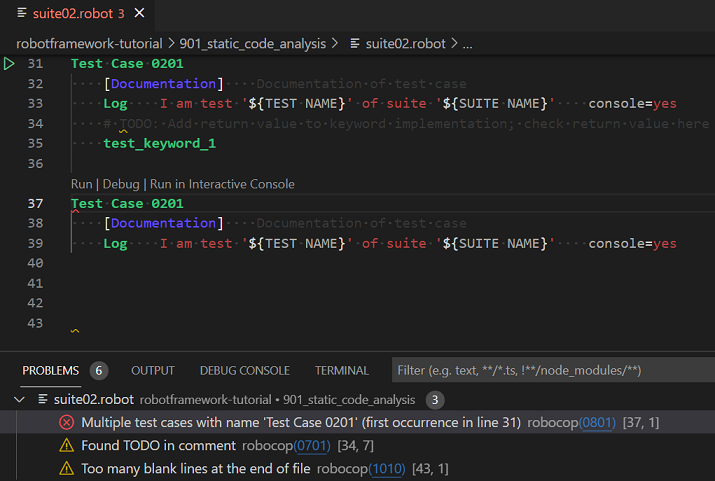
\includegraphics{./include/graphics/code_analysis/Overview}

Further examples can be found in the \rfw\ tutorial, chapter \rlog{901_static_code_analysis}.

\vspace{2ex}

\textbf{How to configure?}

Robocop contains a set of rules that are used to check the source files of the \rfw. Not all of them are really useful and some of them are also against
our company internal development rules. Therefore we have the need to exclude rules from Robocop execution.

Some rules can be configured (e.g. the rule checking the maximum number of characters within a line of code). Also here we have the need for careful adaptions.

When Robocop is triggered automatically within Visual Studio Code, then the configuration is done with the help of a \rlog{.robocop} file. This file has to be placed
within the projects folder (see tutorial). To make Robocop results comparable this configuration file should not be modified - or at least should be kept aligned with
the version all other project team members use.

\newpage

\textbf{Command line}

In addition to the automated triggering within Visual Studio Code Robocop can also be called in command line. This is useful
\begin{enumerate}
   \item in case of a complete folder has to be checked in one step (to avoid the need to open every single source file inside separately),
   \item in case of an alternative configuration is wanted (temporarily; to avoid to manipulate the standard configuration file),
   \item in case of Robocop shall be triggered by automats like Jenkins,
   \item in case of the Robocop results are needed within a log file (output to a log file needs to be configured separately).
\end{enumerate}

To give it a try make a copy of the configuration file \rlog{.robocop} available within the tutorial, and give this copy any other name (e.g. \rlog{robocop.arg}).

Now Robocop can be called with command lines like this:

\vspace{2ex}

\textit{1.) Simple check of single file with default configuration:}

\begin{pythoncode}
"%RobotPythonPath%/python.exe" -m robocop "<\inlinecomment{path}>/mytestfile.robot"
\end{pythoncode}

\vspace{2ex}

\textit{2.) Check of single file with individual configuration taken from argument file:}

\begin{pythoncode}
"%RobotPythonPath%/python.exe" -m robocop --argumentfile "<\inlinecomment{path}>/robocop.arg" "<\inlinecomment{path}>/mytestfile.robot"
\end{pythoncode}

\vspace{2ex}

\textit{3.) Check of entire folder with individual configuration taken from argument file:}

\begin{pythoncode}
"%RobotPythonPath%/python.exe" -m robocop --argumentfile "<\inlinecomment{path}>/robocop.arg" "<\inlinecomment{folder}>"
\end{pythoncode}

\vspace{2ex}

\textbf{How to activate?}

In Visual Studio Code the automated triggering of Robocop is activated per default within

\begin{robotlog}
RobotFramework\robotvscode\data\user-data\User\settings.json
\end{robotlog}

with the following switches set to \rcode{true}:

\begin{pythoncode}
"robot.lint.enabled": true,
"robot.lint.robocop.enabled": true,
\end{pythoncode}

 % ! needs to be reworked !

%  Copyright 2020-2022 Robert Bosch GmbH
%
%  Licensed under the Apache License, Version 2.0 (the "License");
%  you may not use this file except in compliance with the License.
%  You may obtain a copy of the License at
%
%      http://www.apache.org/licenses/LICENSE-2.0
%
%  Unless required by applicable law or agreed to in writing, software
%  distributed under the License is distributed on an "AS IS" BASIS,
%  WITHOUT WARRANTIES OR CONDITIONS OF ANY KIND, either express or implied.
%  See the License for the specific language governing permissions and
%  limitations under the License.
\chapter{Apertis Pro}
\section{How to use DLT}

\subsection{dlt-daemon on Apertis}
Verify that \textbf{dlt-daemon} has installed on Apertis Pro target or not.\\
\rlog{systemctl status dlt-daemon}\\
\\
In case \textbf{dlt-daemon} is not available, follow below steps to install and 
start dlt-daemon service:
\begin{itemize}
   \item Install \textbf{dlt-daemon} package\\
         \rlog{sudo apt install dlt-daemon}
   \item Start \textbf{dlt-daemon} service\\
         \rlog{sudo systemctl start dlt-daemon}
\end{itemize}

\subsection{Apertis Pro firewall configuration}
In order to capture DLT log/trace from DLT client(\textbf{DLT Viewer}, 
\textbf{DLTConnector}), DLT client has to communicate with Apertis Pro  
(TCP/IP protocol) via port \textbf{3490} (as default).\\
So that, this connection should be allowed on Apertis Pro target.\\
\\
Adopt settings of firewall at Apertis Pro:
\begin{itemize}
   \item Add new rule to allow DLT service at port \textbf{3490} (as default)\\
   Edit \rlog{/etc/iptables/rules.v4} file to add below line
   \begin{robotcode}
...
# Accept dlt for development
-A INPUT -p tcp -m state --state NEW -m tcp --dport 3490 -j ACCEPT
...
   \end{robotcode}

   \item Restart the firewall with changed parameters\\
   \rlog{sudo systemctl restart iptables.service}
\end{itemize}

\subsection{DLTSelfTestApp}
\href{https://sourcecode.socialcoding.bosch.com/projects/ROBFW/repos/selftest/browse/helpers/DLT}
{DLTSelfTestApp} is an application which will be run on the Apertis Pro target for 
testing the DLT connection between \rfw\ and target.\\
This package is a part of \rfw\ selftest helpers.\\
To install \textbf{DLTSelfTestApp}, download its debian package on Apertis Pro
target then execute the below command.\\
\rlog{sudo dpkg -i <path/to/dltselftestapp_1.0.0_amd64.deb>}\\
\\
\textbf{DLTSelfTestApp} application will be installed in 
\rlog{/opt/bosch/robfw/dlt} directory and can be started with below command:\\
\rlog{/opt/bosch/robfw/dlt/DLTSelfTestApp}\\
\\
Welcome log message \rlog{Welcome to RobotFramework AIO DLTSelfTestApp...} 
will be sent at application startup.\\
Then the ping log \rlog{ping message from RobotFramework AIO DLTSelfTestApp} 
every 5 seconds.\\
\\
\textbf{\underline{DLT command injection:}}\\
To perform the DLT command injection, use below information:
\begin{itemize}
   \item App ID: \textbf{RBFW}
   \item Context ID: \textbf{TEST}
   \item Service ID: \textbf{0x1000}
   \item Data as Textdata
\end{itemize}

DLT log reponse of \textbf{DLTSelfTestApp} will bases on injected command:
\begin{itemize}
   \item \rcode{welcome}: DLT reponse as above welcome message.
   \item \rcode{exit}: DLT reponse as \rlog{Bye...} then \textbf{DLTSelfTestApp} 
                       will be terminated.
   \item Other commands: DLT reponse as combination of data and string.\\
   e.g: \rlog{Data: 000000: 77 65 6c 63 6f 6d 65 31 32 31 32 00 xx xx xx xx 
              welcome1212}
\end{itemize}

\subsection{QConnectDLTLibrary}
\href{https://sourcecode.socialcoding.bosch.com/projects/ROBFW/repos/robotframework-qconnect-dlt/browse}
{QConnectDLTLibrary} is part of \rfw.
It provides the ability for handling connection to Diagnostic Log and Trace(DLT) Module. 
The library support for getting trace message and sending trace command\\
\\
Sample \rfw\ testcase which are using \textbf{QConnectDLTLibrary} to 
test DLTSelfTestApp on Apertis Pro target:
\begin{itemize}
   \item Header of a \rfw\ testcase containing common settings (\rcode{*** Settings ***}) like the setups and teardowns,
         the definition of variables (\rcode{*** Variables ***})
         and the definition of keywords (\rcode{*** Keywords ***}):
   \begin{robotcode}
*** Settings ***
Documentation  This is selftest for DLT connection with DLTSelfTestApp
Library     QConnectionLibrary.ConnectionManager 
Suite Setup     Open Connection
Suite Teardown  Close Connection

*** Variables ***
${CONNECTION_NAME}  TEST_CONN_DLTSelfTestApp
${DLT_CONNECTION_CONFIG} =  SEPARATOR=
...  {
...      "gen3flex@DLTLSIMWFH": {
...            "target_ip": "127.0.0.1",
...            "target_port": 4490,
...            "mode": 0,
...            "ecu": "ECU1",
...            "com_port": "COM1",
...            "baudrate": 115200,
...            "server_ip": "localhost",
...            "server_port": 1234
...      }
...  }

*** Keywords ***
Close Connection
   disconnect  ${CONNECTION_NAME}
   Log to console    \nDLT connection has been closed!

Open Connection
   ${dlt_config} =    evaluate    json.loads('''${DLT_CONNECTION_CONFIG}''')   json

   connect             conn_name=${CONNECTION_NAME}
   ...                 conn_type=DLT
   ...                 conn_mode=dltconnector
   ...                 conn_conf=${dlt_config}

   Log to console    \nDLT connection has been opened successfully!
   \end{robotcode}

   \item Sample \rfw\ testcase to verify the ping message from DLTSelfTestApp
   \begin{robotcode}
*** Test Cases ***
Match log/trace from DLTSelfTestApp
   [Documentation]   Match log/trace from DLTSelfTestApp
   [Tags]   DLTSelfTestApp
   ${res}=    verify     conn_name=${CONNECTION_NAME}
   ...                   search_pattern=(DLT:0x01.*RBFW.*)
   ...                   timeout=6    # DLTSelfTestApp pings a message every 5 seconds

   # log to console     \n${res}[0]
   # verify that reponse message should contain "Ping" keyword
   Should Match Regexp     ${res}[0]    DLT:0x01.*RBFW.*Ping.*   
   \end{robotcode}

   \item Sample \rfw\ testcase to verify command injection with DLTSelfTestApp
   \begin{robotcode}
Command injection with DLTSelfTestApp
   [Documentation]   Get log/trace from DLTSelfTestApp
   [Tags]   DLTSelfTestApp
   ${res}=    verify     conn_name=${CONNECTION_NAME}
   ...                   search_pattern=(DLT:0x01.*RBFW.*Welcome.*)
   ...                   send_cmd=DLT_CALL_SW_INJECTION_ECU ECU1 1000 RBFW TEST 'welcome'

   # log to console     \n${res}[0]

   ${res}=    verify     conn_name=${CONNECTION_NAME}
   ...                   search_pattern=(DLT:0x01.*RBFW.*other_cmd.*)
   ...                   send_cmd=DLT_CALL_SW_INJECTION_ECU ECU1 1000 RBFW TEST 'other_cmd'

   # log to console     \n${res}[0]
   \end{robotcode}
\end{itemize}

Please refer \href{https://sourcecode.socialcoding.bosch.com/projects/ROBFW/repos/robotframework-qconnect-dlt/browse}
{QConnectDLTLibrary repository} for more details about usage and other 
example testcase for DLT connection.

% --------------------------------------------------------------------------------------------------------------

\chapter{Library documentation}

The following sections contain the documentation of additional libraries that are part of the RobotFramework AIO.

Overview about the included libraries:

% --------------------------------------------------------------------------------------------------------------
% document content (automatically generated part)
%
% following input files require the execution of genmaindoc.py, otherwise they are not available
% --------------------------------------------------------------------------------------------------------------

\begin{center}
\begin{tabular}{| m{44em} |}\hline
   \textbf{PythonExtensionsCollection}\\ \hline
   Version 0.7.3 (from 24.06.2022)\\ \hline
   https://github.com/test-fullautomation/python-extensions-collection\\ \hline
   \textit{Additional Python functions}\\ \hline
\end{tabular}

\vspace{2ex}

\begin{tabular}{| m{44em} |}\hline
   \textbf{RobotframeworkExtensions}\\ \hline
   Version 0.6.2 (from 24.06.2022)\\ \hline
   https://github.com/test-fullautomation/robotframework-extensions-collection\\ \hline
   \textit{Additional Robot Framework keywords}\\ \hline
\end{tabular}

\vspace{2ex}

\begin{tabular}{| m{44em} |}\hline
   \textbf{GenPackageDoc}\\ \hline
   Version 0.18.1 (from 24.06.2022)\\ \hline
   https://github.com/test-fullautomation/python-genpackagedoc\\ \hline
   \textit{Documentation builder for Python packages}\\ \hline
\end{tabular}

\vspace{2ex}

\end{center}



% Generated at 30.06.2022 - 15:03:32
%
% This document imports the documentation of additional RobotFramework AIO libraries into the main documentation.
%
% The split of the \includepdf for a single PDF file is a workaround to avoid a linebreak after the section heading
% (one \newpage too much within pdfpages.sty).
%

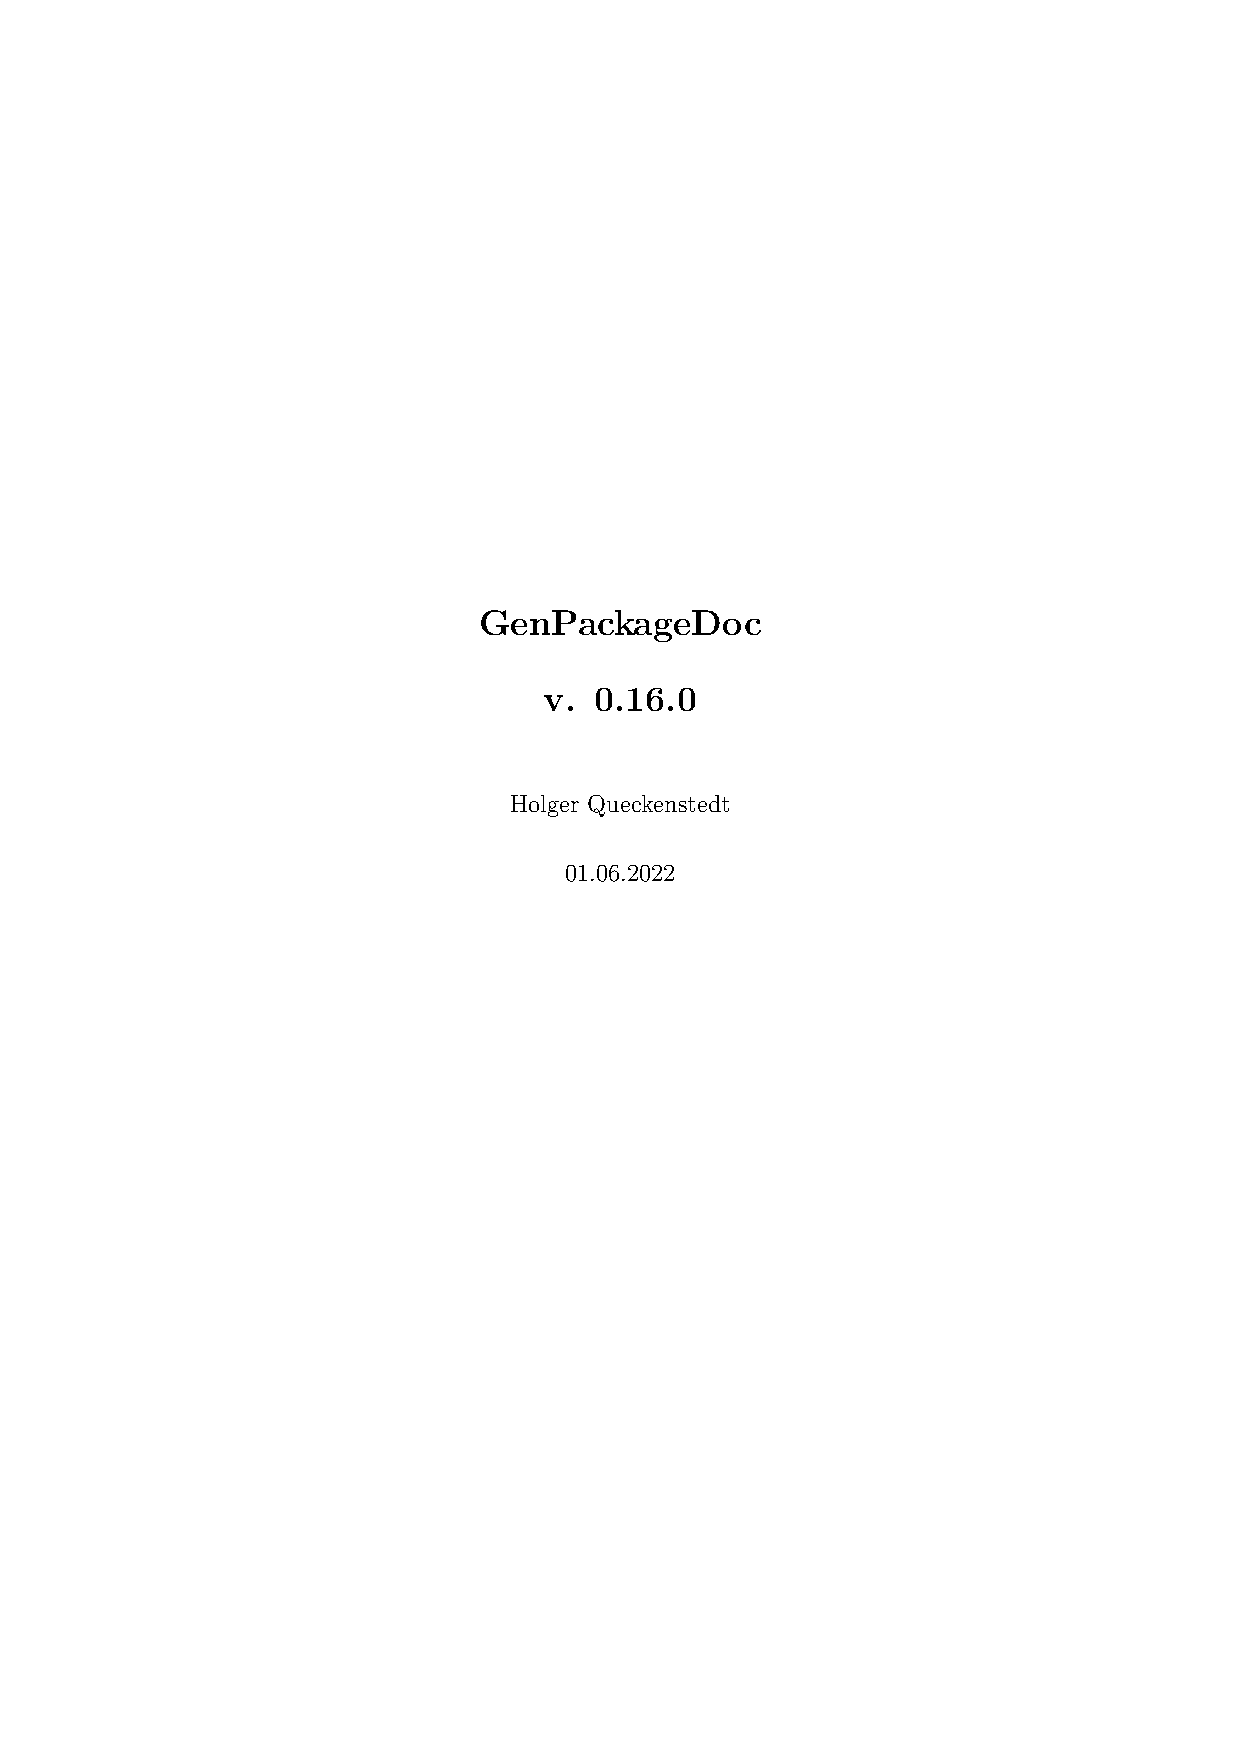
\includepdf[pages=1,pagecommand=\section{GenPackageDoc}]{./include/libraries/python-genpackagedoc/GenPackageDoc.pdf}
\includepdf[pages=2-,pagecommand={}]{./include/libraries/python-genpackagedoc/GenPackageDoc.pdf}
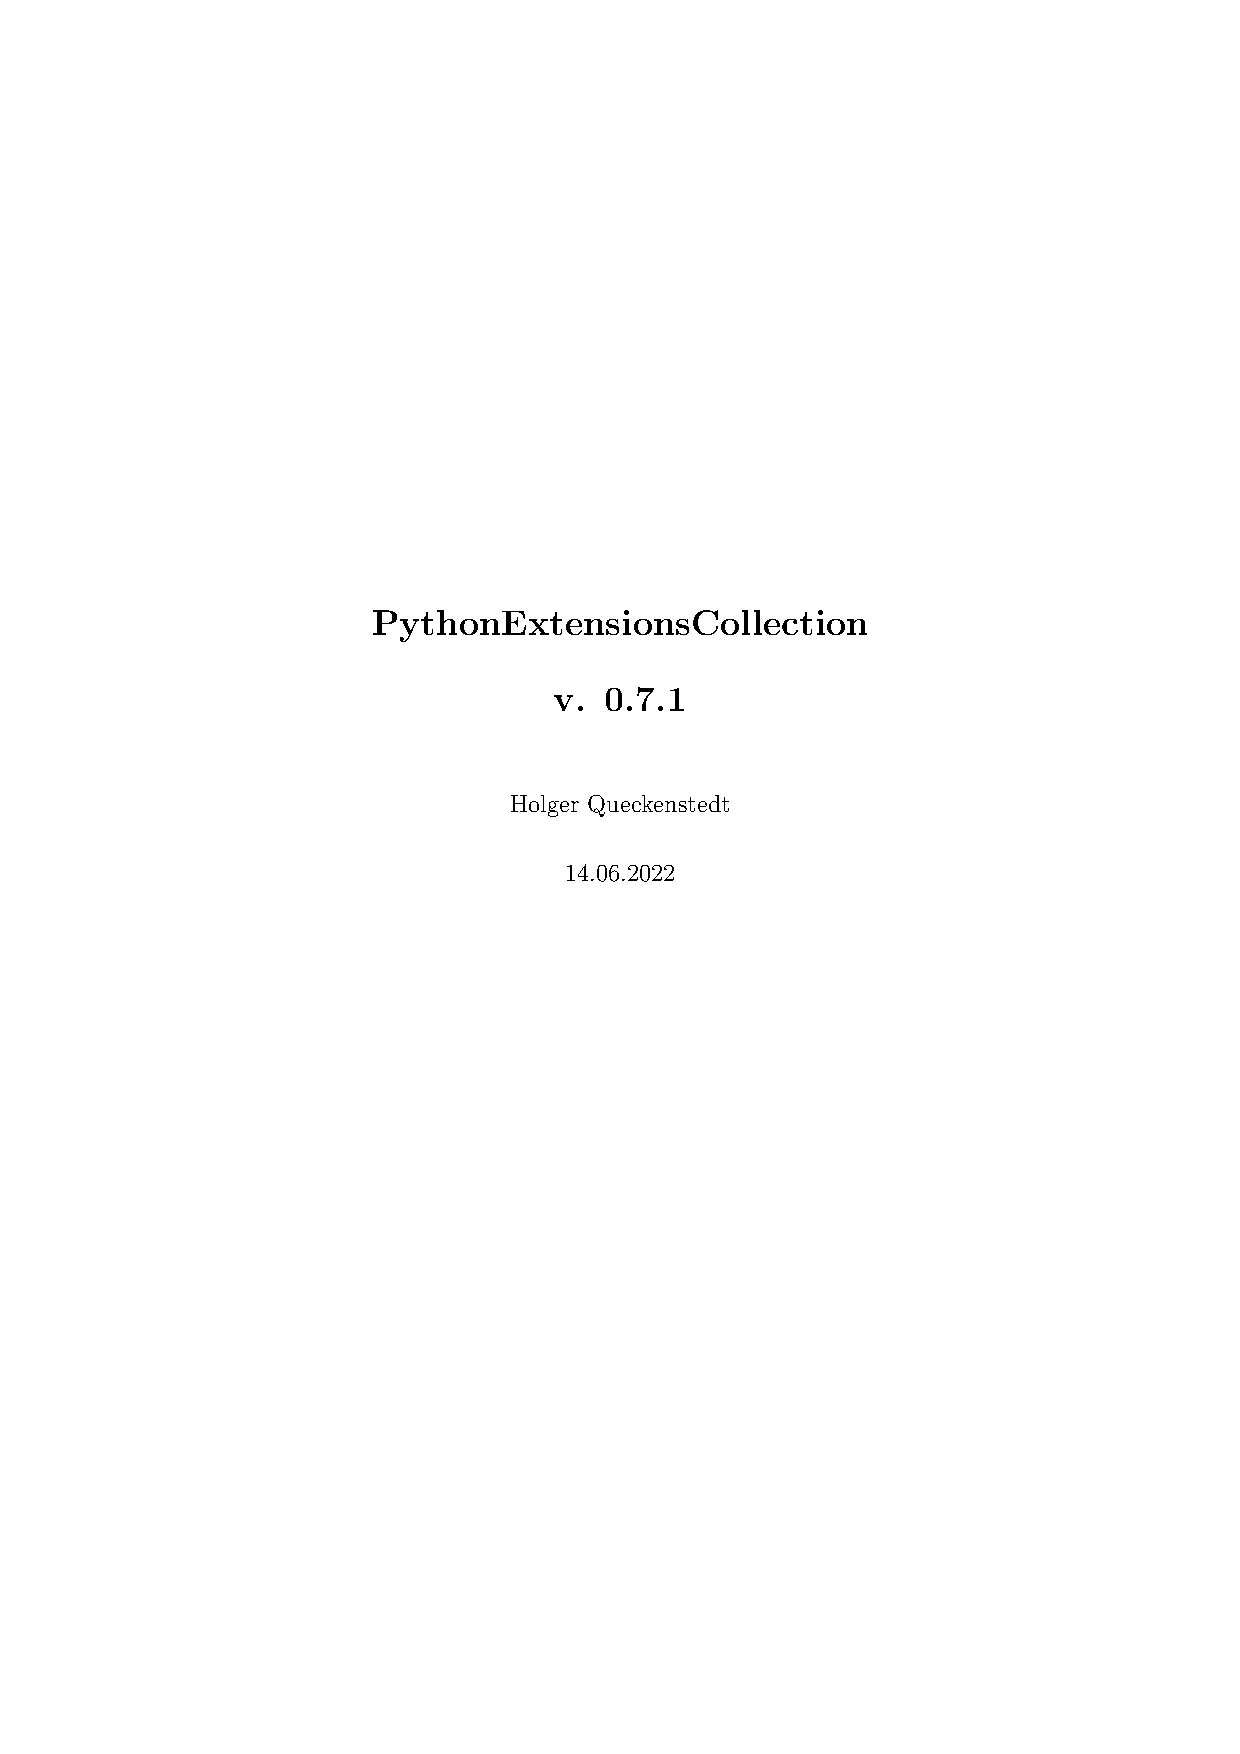
\includepdf[pages=1,pagecommand=\section{PythonExtensionsCollection}]{./include/libraries/python-extensions-collection/PythonExtensionsCollection.pdf}
\includepdf[pages=2-,pagecommand={}]{./include/libraries/python-extensions-collection/PythonExtensionsCollection.pdf}
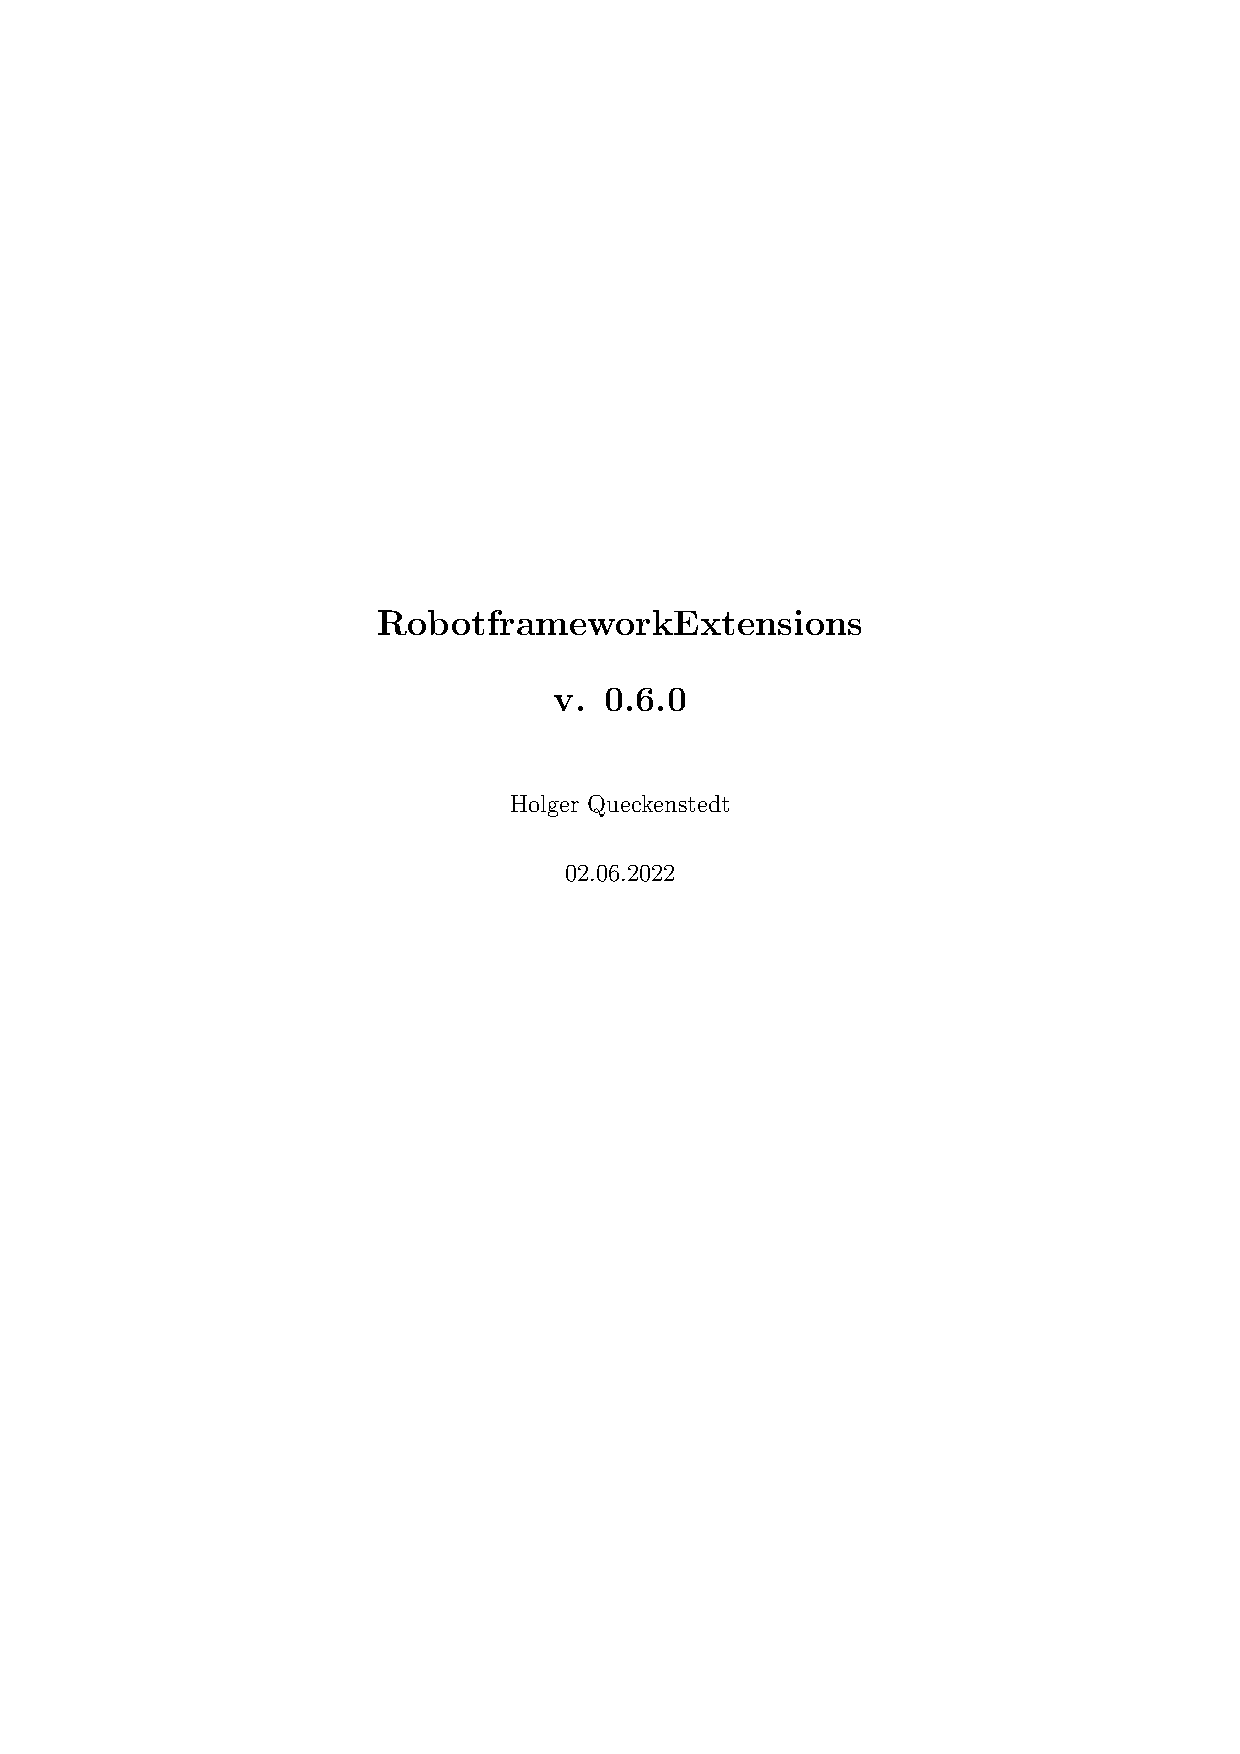
\includepdf[pages=1,pagecommand=\section{RobotframeworkExtensions}]{./include/libraries/robotframework-extensions-collection/RobotframeworkExtensions.pdf}
\includepdf[pages=2-,pagecommand={}]{./include/libraries/robotframework-extensions-collection/RobotframeworkExtensions.pdf}
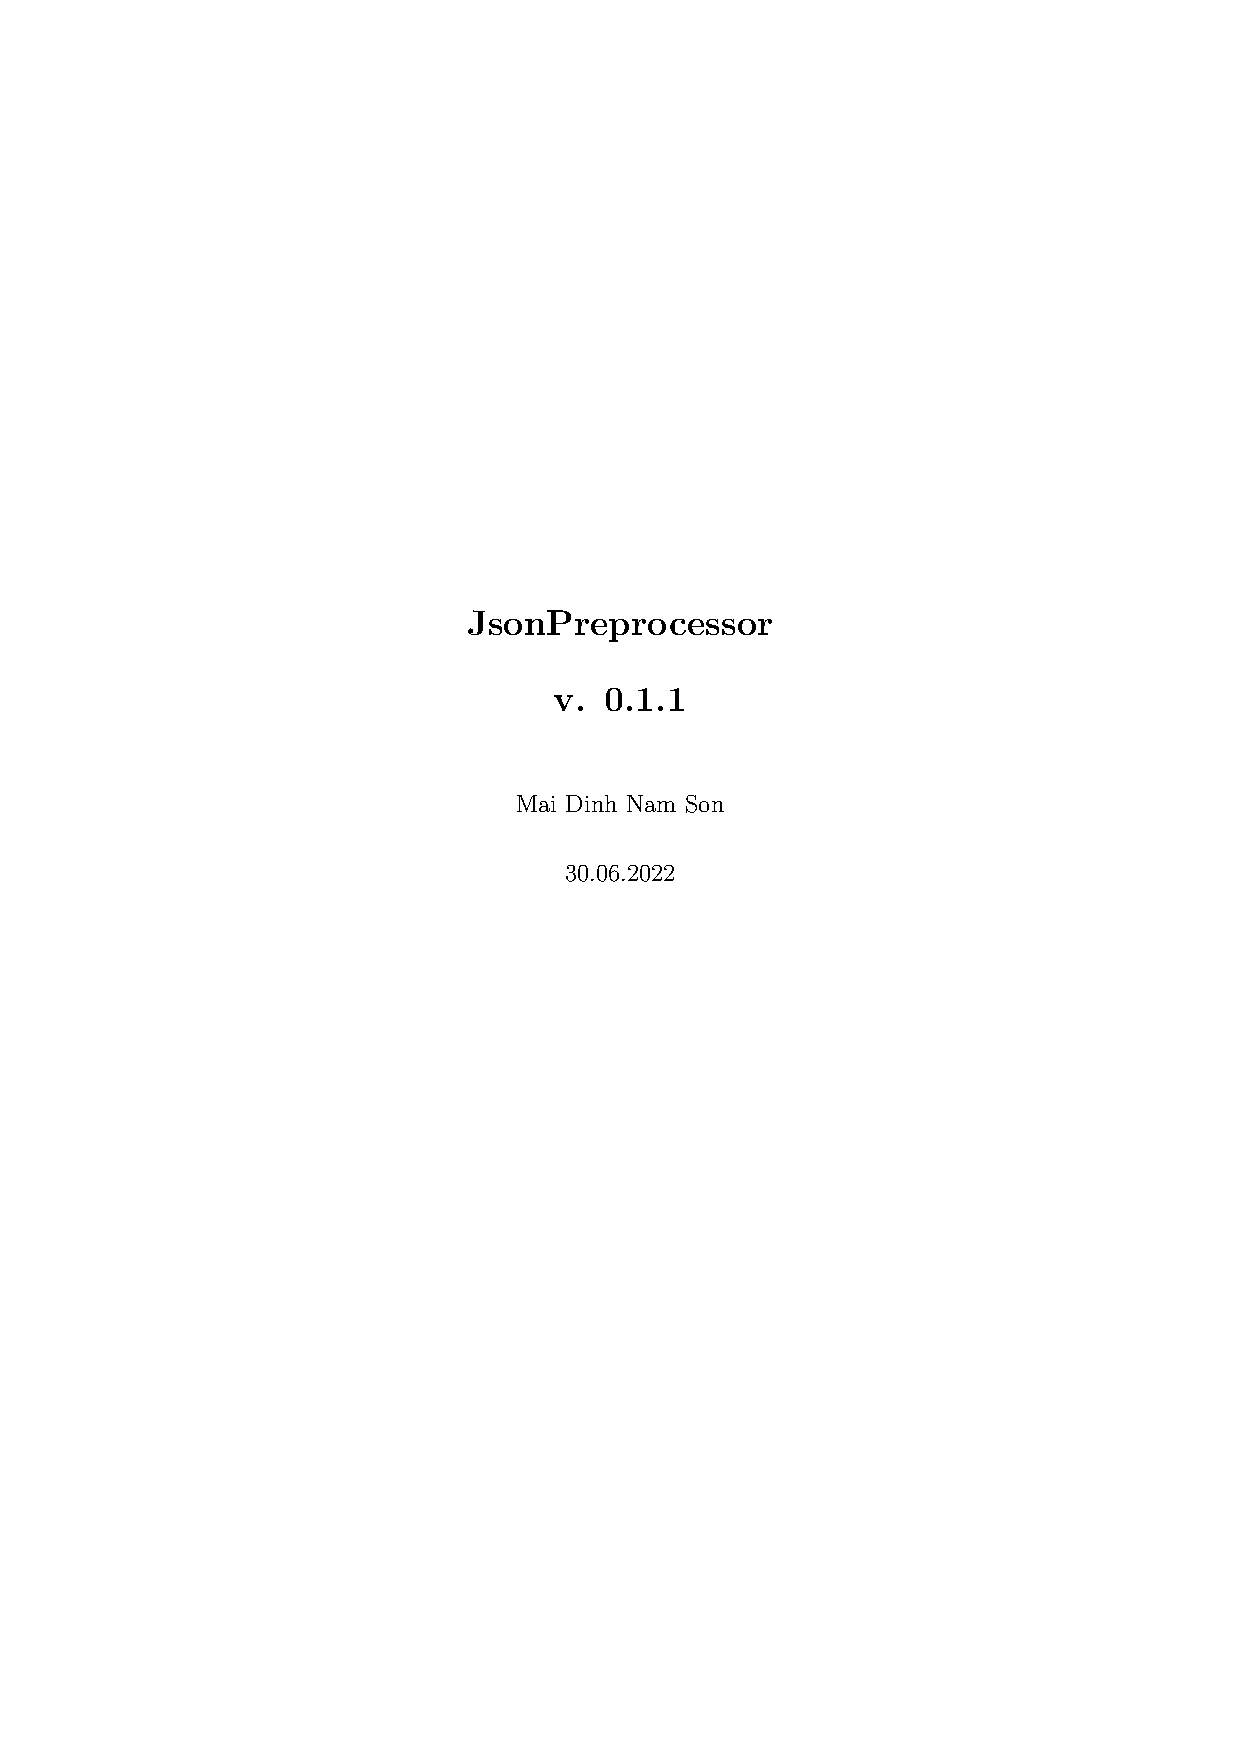
\includepdf[pages=1,pagecommand=\section{JsonPreprocessor}]{./include/libraries/python-jsonpreprocessor/JsonPreprocessor.pdf}
\includepdf[pages=2-,pagecommand={}]{./include/libraries/python-jsonpreprocessor/JsonPreprocessor.pdf}
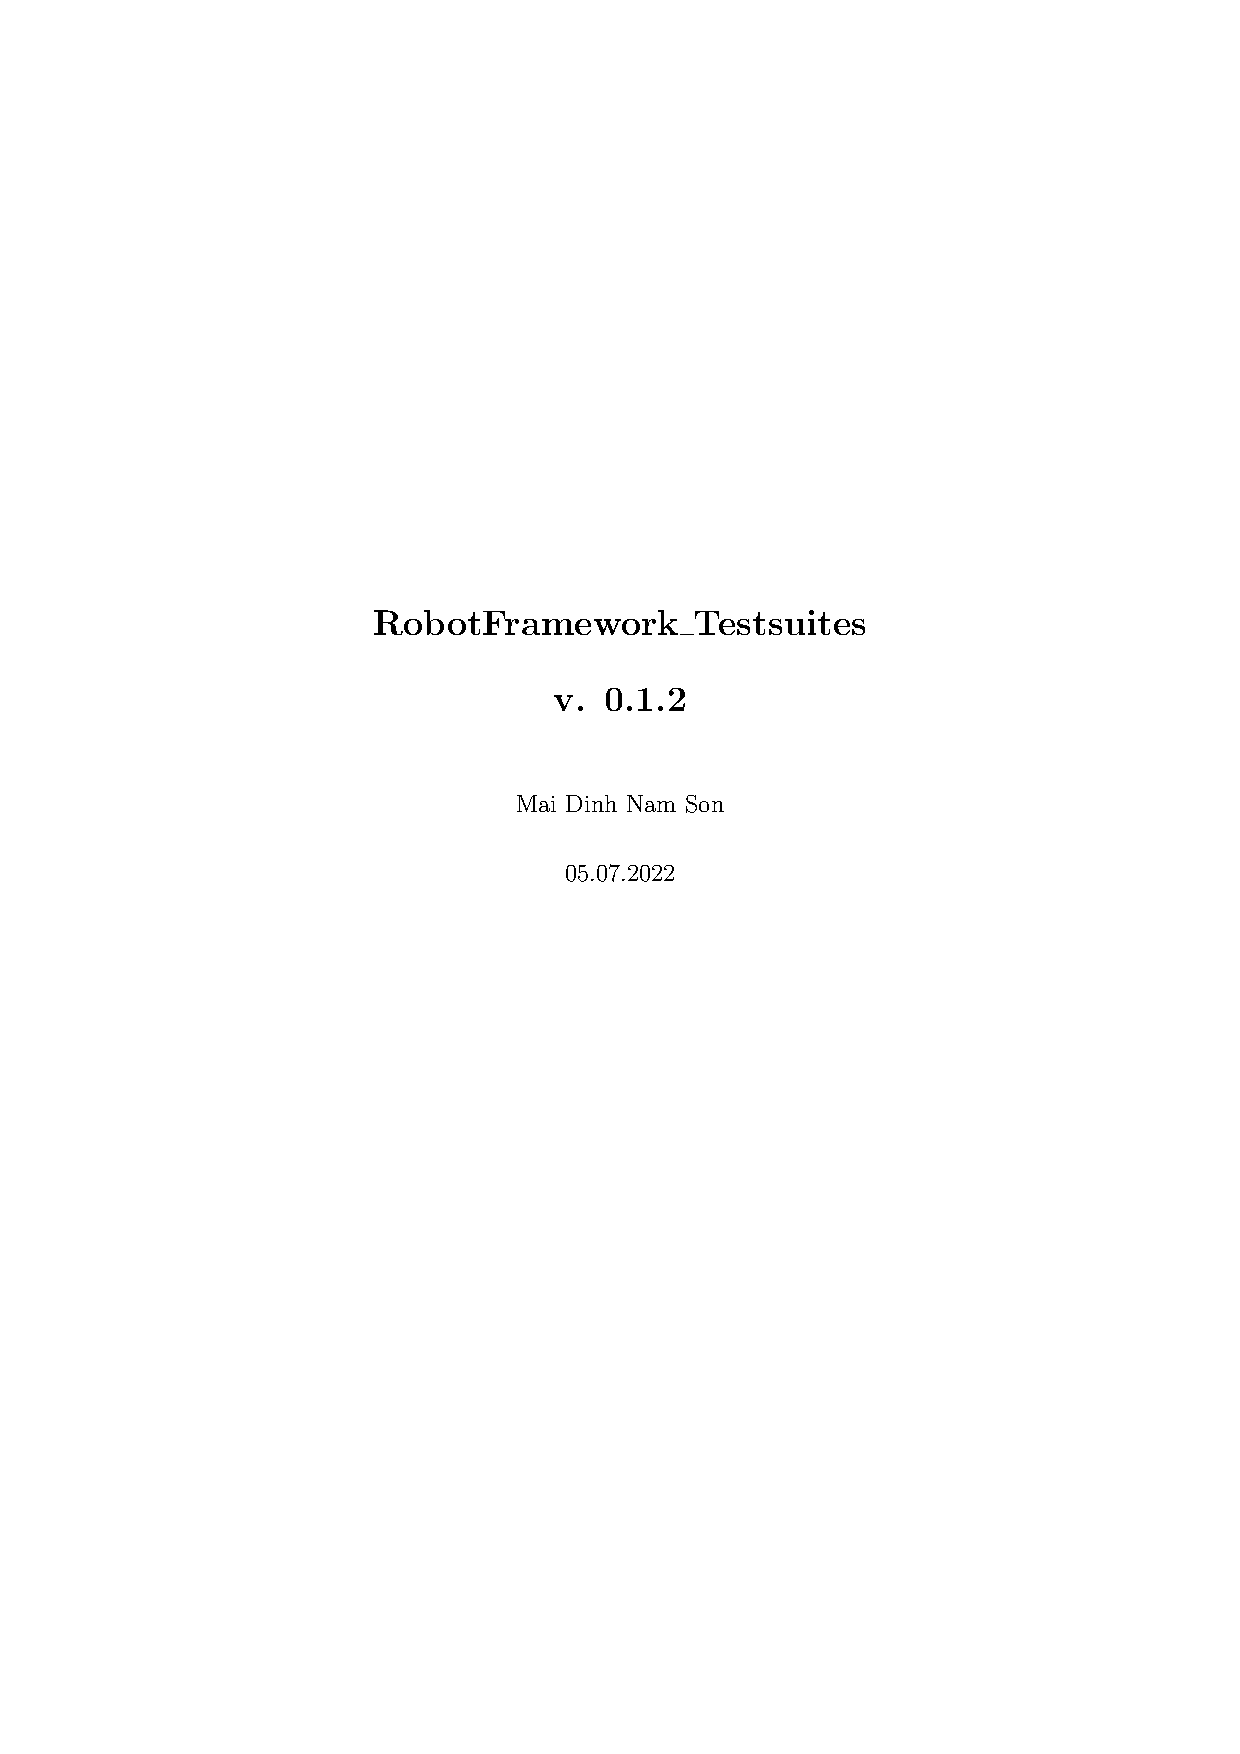
\includepdf[pages=1,pagecommand=\section{RobotFramework\_Testsuites}]{./include/libraries/robotframework-testsuitesmanagement/RobotFramework_Testsuites.pdf}
\includepdf[pages=2-,pagecommand={}]{./include/libraries/robotframework-testsuitesmanagement/RobotFramework_Testsuites.pdf}


% --------------------------------------------------------------------------------------------------------------
% appendix
% --------------------------------------------------------------------------------------------------------------

%\backmatter
%glossary and index would go here.

\end{document}
